\documentclass[11pt,a4paper]{article}
\usepackage[margin=2.5cm]{geometry}
\usepackage[T1]{fontenc}
\usepackage{lmodern}
\usepackage{booktabs,tabularx,longtable,array,enumitem}
\usepackage{tikz}
\usetikzlibrary{positioning,arrows.meta}

\usepackage{float}
\usepackage[hidelinks]{hyperref}


\setlist{itemsep=2pt,topsep=4pt}
\newcolumntype{L}{>{\raggedright\arraybackslash}X}
\renewcommand{\arraystretch}{1.15}
\newcommand{\eps}{\varepsilon}

\title{\textbf{Follow the Money Without Moving the Data}\\[4pt]
\large Catching money laundering across banks by asking small, private, tested questions\\[2pt]
\large Mid-Submission Status Report}
\author{Team \textbf{Cache me if you can} \quad LMA Group Project 2026\\[6pt]
G Sai Abhishek (2023113005) \quad Bhavya Ram V (2023114013)\\
Shreyas Deb (2023113024) \quad Akshat Srivastava (2023111020)\\[6pt]
\small Code: \url{https://github.com/BhavyaV05/Transaction-Thieves}}
\date{30 October 2026}

\begin{document}
\maketitle

\begin{abstract}
\noindent This report gives the state of the project at the mid-submission point, eleven days before the final deadline of 10 November 2026. The system lets a bank that is unsure about a transaction alert ask partner banks a small number of privacy-protected questions, written in a restricted query language, and combines the noisy answers with its own model through likelihood ratios that were estimated in advance on past alerts. All components of the pipeline are implemented and tested (1,348 automated tests), and every model and agent has been run on real validation data from the IBM AMLworld HI-Small and HI-Medium datasets. The test split is locked in code and has not been read; the final test run starts after the pre-registration is frozen on 30 October. On validation, the one-bank versus see-everything gap that motivates the project is confirmed on both datasets, while the expert questions, under the naive fusion rule, fall short of the Brier improvement that the pre-registered gate G2 requires. Fitted per-family fusion moves the score in the right direction, with an interval that still includes zero.
\end{abstract}

\section{Introduction}

Each bank sees only the transactions that touch its own customers, while laundered money is routed through accounts at many banks. The authors of the AMLworld dataset showed that a model restricted to one bank's slice of the transaction graph detects far less than a model that sees the whole graph \cite{altman2023}. Banks cannot pool their data, but regulations such as Section 314(b) in the United States allow them to ask each other about specific accounts \cite{cfr314b}. In practice this usually means sending transaction records, which is slow and discloses a large amount of customer data.

The project studies a more private alternative. For an alert its own model is unsure about, a bank sends partner banks a few questions, each answered with one small value perturbed by differential-privacy noise (for example, whether an account forwarded more than 80\% of what it received within 24 hours). The questions are written in a small domain-specific language (DSL) that partner banks execute on their own data. The strength of each question is estimated in advance by back-testing it on past alerts with the same noise, so its answer can be turned into a likelihood ratio. A planner chooses the questions within a per-alert privacy budget ($\eps = 2$). The planner is either a large language model (LLM) or one of several non-LLM baselines.

The project asks three questions:
\begin{enumerate}
\item How much of the one-bank versus see-everything gap such questions recover at a fixed privacy budget, and how this compares with sharing raw records and with privacy-preserving federated training.
\item Whether an LLM composing questions does better than simple question pickers and than existing LLM investigation agents on the same backbone.
\item Which parts of the system (back-testing, retrieval of evidence, the decision formula, a fast model for routine decisions, asynchronous questioning) contribute.
\end{enumerate}
The ten hypotheses (H1--H10) and eighteen experiments (E1--E18) are pre-registered in the repository (\texttt{prereg/hypotheses.yaml}, \texttt{plan.md}). Figure~\ref{fig:arch} shows the pipeline.

\begin{figure}[h]
\centering
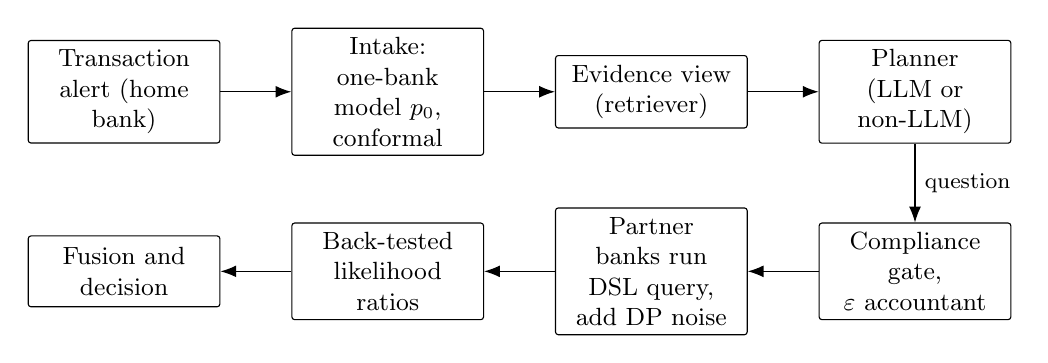
\begin{tikzpicture}[node distance=6mm and 9mm, every node/.style={font=\small},
  box/.style={draw, rounded corners=1pt, align=center, minimum height=9mm, text width=22mm},
  arr/.style={-{Latex[length=2mm]}}]
\node[box] (alert) {Transaction\\alert (home bank)};
\node[box, right=of alert] (intake) {Intake: one-bank\\model $p_0$, conformal};
\node[box, right=of intake] (evid) {Evidence view\\(retriever)};
\node[box, right=of evid] (plan) {Planner\\(LLM or non-LLM)};
\node[box, below=10mm of plan] (gate) {Compliance gate,\\$\eps$ accountant};
\node[box, left=of gate] (banks) {Partner banks run\\DSL query, add DP noise};
\node[box, left=of banks] (bt) {Back-tested\\likelihood ratios};
\node[box, left=of bt] (fus) {Fusion and\\decision};
\draw[arr] (alert) -- (intake);
\draw[arr] (intake) -- (evid);
\draw[arr] (evid) -- (plan);
\draw[arr] (plan) -- node[right, font=\footnotesize]{question} (gate);
\draw[arr] (gate) -- (banks);
\draw[arr] (banks) -- (bt);
\draw[arr] (bt) -- (fus);
\end{tikzpicture}
\caption{Pipeline for one alert. After each answer the posterior is updated and returned to the planner, which repeats the question step until the budget is spent or no remaining question can move the decision.}
\label{fig:arch}
\end{figure}


\section{Progress Summary}

All planned components are implemented, merged into the main branch and covered by tests. Table~\ref{tab:progress} gives the status of each component as of 30 October. ``Run on real data'' means a run on the HI-Small or HI-Medium training and validation splits; no component has been run on the test split.

\begin{table}[!htbp]
\centering\small
\begin{tabularx}{\textwidth}{@{}p{3.6cm}LL@{}}
\toprule
Component & Implemented & Run on real validation data \\
\midrule
Data pipeline and test lock & Parquet build, time-based splits, 30 bank views per dataset, aliasing, guarded readers & Both datasets built \\
Intake & GFP+LightGBM one-bank model, Mondrian conformal alert rule & Train and val alert sets, both datasets \\
Detection baselines & GFP, Multi-GNN, MEGA-GNN, FraudGT, DP-FedAvg (two privacy units), layer-wise federated exchange & All run; see Section~\ref{sec:baselines} \\
Retrieval & Edge scorer, time-respecting PCST trail, four evidence views, three graph explainers & Both datasets \\
Query language & DSL v0: 24 primitives, parser, type checker, executor checked against a brute-force reference & 110 expert programs \\
Partner banks and privacy & Simulated banks with latency, declines and timeouts; DP mechanisms with exact likelihoods; per-alert and per-account accountant & Used in every real run \\
Back-testing & Label-permutation e-values, e-BH and e-LOND acceptance, realistic and exact modes, time blocks & Realistic table: 23 of 440 hypotheses accepted (HI-Medium) \\
Harness & Gate, accountant and clock in front of every question; version 1.0 frozen with a contract test & Used in every real run \\
Non-LLM planners & Random, fixed order, EIG, learned policy, enumerator & 18 of 19 arms on HI-Medium val \\
LLM planner & Five planner modes, JSON schema, retries, stop rules, strategy library, batching & Backbone sweep (E18), evidence views (E8), teacher runs \\
External agents & 15 systems ported or reimplemented (Table~\ref{tab:agents}) & ReAct and the Group C/D ports on Gemma 4 12B; full table in progress \\
Fine-tuning & Distillation filter, QLoRA trainer, fast model, conformal cascade & Training sets built; training queued \\
Fusion, decision, compliance & Naive, shared and per-family fusion; threshold and stop rule; gate with a 44-flag red-flag corpus & Fusion diagnostics on both datasets \\
Safety & Injection set (400 attacks, 400 benign notes), CaMeL-style comparison & Mock LLM only \\
Evaluation and final run & Metrics, cluster bootstrap, Holm correction, run-log v1, final-run orchestrator, pre-registration freeze, final analysis & Dry runs on synthetic data and val \\
\bottomrule
\end{tabularx}
\caption{Component status, 30 October 2026.}
\label{tab:progress}
\end{table}

The project gates are defined in \texttt{plan.md}. G0 (setup, machine reports) and G1 (data and baselines reproduced) are complete. G3 (frozen subset rule, external-agent list and harness contract) is complete. G2, which requires the expert questions to improve the Brier score by at least 0.01 on validation, is \emph{not met} on real data; Section~\ref{sec:results} gives the numbers, and Section~\ref{sec:mitigation} the decision that follows from it. G4, the validation table of all systems and the choice of the external agents for the full test set, and the freeze of the pre-registration are due on 30 October. The backbone decision (E18), which the pre-registration required before the final run, was committed on 26 October.

The codebase consists of about 24,700 lines of Python in the \texttt{ftm} package, 7,600 lines of scripts and 85 test files with 1,348 tests. The full test suite runs in continuous integration on every pull request.

\section{Datasets}

\subsection{IBM AMLworld}

The project uses two synthetic datasets from IBM AMLworld \cite{altman2023}, both from the high-illicit (HI) setting. In AMLworld every transaction is labelled, and laundering transactions are grouped into attempts with a known typology. Table~\ref{tab:data} gives the statistics computed from the built files. Test-split label counts are not reported, in line with the test lock.

\begin{table}[!htbp]
\centering\small
\begin{tabular}{@{}lrr@{}}
\toprule
 & HI-Small & HI-Medium \\
\midrule
Transactions & 5,078,345 & 31,898,238 \\
Laundering transactions & 5,177 (0.102\%) & 35,230 (0.110\%) \\
Accounts & 518,581 & 2,087,786 \\
Calendar days & 18 & 28 \\
Split days (train / val / test) & 1--6 / 7--8 / 9--18 & 1--9 / 10--12 / 13--28 \\
Train transactions (laundering) & 3,248,921 (2,530) & 19,487,126 (15,713) \\
Val transactions (laundering) & 965,524 (1,036) & 3,592,257 (6,226) \\
Test transactions & 863,900 & 8,818,855 \\
Laundering attempts & 370 & 2,756 \\
Attempts spanning a split boundary & 147 & 1,046 \\
Share of transactions in the 30 modelled bank views & 32.9\% & 19.5\% \\
Share of laundering transactions in those views & 38.3\% & 26.8\% \\
\bottomrule
\end{tabular}
\caption{Dataset statistics (\texttt{ftm/data/README.md}, from the build manifests).}
\label{tab:data}
\end{table}

Eight typologies are present: fan-in, fan-out, cycle, scatter-gather, gather-scatter, bipartite, stack and random. They are close to balanced, with 40 to 54 attempts per typology in HI-Small and 322 to 369 in HI-Medium. Not every laundering transaction belongs to a recorded attempt: 1,968 of the 5,177 in HI-Small and 12,487 of the 35,230 in HI-Medium have no attempt, so ``not in an attempt'' is never read as ``clean''. HI-Medium is the headline dataset of the final run; HI-Small is used for development and reproductions.

\subsection{Splits, bank views and alert sets}

The splits are by time (Table~\ref{tab:data}). The HI-Medium test split keeps a sparse tail after the 16 bulk days, so that time order holds; the headline test numbers will use the bulk days, and the tail will be reported separately. The validation split is divided in time order into \texttt{fit}, \texttt{cal} and \texttt{eval} parts, used for fitting fusion parameters, calibrating thresholds and reporting validation numbers respectively.

Each of the 30 largest banks by transaction count is modelled as a separate institution. Its view contains only the transactions it sends or receives, and its one-bank model is trained on that view alone. Account identifiers shown to any LLM are replaced by aliases.

Alerts are produced by the intake: a one-bank GFP+LightGBM model gives the probability $p_0$ that a transaction is laundering, and a Mondrian split-conformal rule, calibrated on the validation \texttt{cal} part, marks the transactions the bank is unsure about. With the chosen setting, HI-Medium yields 10,962 training alerts and 2,238 validation alerts. Of the latter, 460 are \emph{askable}, meaning the alert has a partner bank among the 30 modelled banks (191 \texttt{fit}, 109 \texttt{cal}, 160 \texttt{eval}). The test alert count is projected from the validation rate at 3,475 alerts with about 1,011 positives. This is a projection, not a measurement.

\subsection{Test lock and held-out variants}

The test split is locked in code. Every data reader requires a split or a time cut-off, and a request for test rows raises an error unless the environment variable \texttt{FTM\_FINAL\_RUN=1} is set. This variable is set only by the final-run orchestrator, after the pre-registration hashes have been checked. A static test fails if any tool reads the data files without going through the guarded reader. Every feature, view and question answer uses only data with a timestamp at or before the alert time. For experiment E12, a held-out-cycles variant of both datasets removes the transactions of cycle attempts from training and back-testing. A synthetic world with the same interfaces is used for unit tests and dry runs.

\section{Baseline Experiments}
\label{sec:baselines}

\subsection{Detection models (Groups A and B)}

Each detection model is trained in two modes. \emph{One-bank} models use one bank's view only and give the starting probability $p_0$. \emph{See-everything} models use the whole graph and serve as the upper limit. Federated models train across the 30 banks without pooling data.

\paragraph{Reproductions on the original splits.} Before running on the project split, three models were reproduced on the splits of their original papers (Table~\ref{tab:repro}). These reproductions use the original papers' own splits on the raw files. Their test periods overlap the project's test days, so nothing from them feeds any model, score, threshold or decision of the project.

\begin{table}[!htbp]
\centering\small
\begin{tabularx}{\textwidth}{@{}lccL@{}}
\toprule
Model & Reproduced F1 & Published F1 & Notes \\
\midrule
GFP + LightGBM \cite{blanusa2024} & 62.95 & 62.86 & XGBoost variant 62.51 vs 63.23 \\
Multi-GNN (Multi-PNA+EU) \cite{egressy2024} & 67.64 & 68.16 & 5 of 100 epochs in a 2.5 h budget \\
MEGA-GNN (MEGA-GenAgg) \cite{bilgi2024} & 59.7 & 74.88 & Partial: 10 of 80 epochs in the same 2.5 h budget \\
FraudGT \cite{lin2024} & val F1 0.648 & -- & Partial: 111 of 500 epochs in 3 h; full run in progress \\
\bottomrule
\end{tabularx}
\caption{Reproductions on the original papers' splits (HI-Small).}
\label{tab:repro}
\end{table}

\paragraph{Baselines on the project split.} All models were trained on the project's training split and evaluated on the validation \texttt{eval} part. Metrics are computed on (transaction, bank view) rows. Confidence intervals come from a cluster bootstrap over laundering attempts and accounts, with a cap on hub accounts. The models are:
\begin{itemize}
\item a constant predictor at the training base rate;
\item GFP+LightGBM, Multi-GNN and MEGA-GNN, one-bank and see-everything;
\item DP-FedAvg \cite{mcmahan2018} over the 30 bank views, with two privacy units: client-level, where the unit is a bank, at $\eps \in \{1,2,4,8,16,\infty\}$, and edge-level, where the unit is a transaction, at $\eps \in \{1,2,4,8,\infty\}$;
\item the layer-wise federated exchange of Ceydeli et al.\ \cite{ceydeli2026}, implemented from the paper with eight arms and three seeds. It replaces the AML-specific method of Tian et al.\ \cite{tian2025}, whose code has no licence.
\end{itemize}

\subsection{Retrieval baselines}

The LLM receives up to 40 edges of evidence per alert. Four evidence views were built:
\begin{itemize}
\item the top 40 edges by amount within one hop;
\item the top 40 by a learned edge scorer;
\item the scorer plus a time-respecting prize-collecting Steiner tree (PCST) trail;
\item all candidate edges serialised up to a 4,000-token cap.
\end{itemize}
Three graph explainers were added for comparison: personalised PageRank, GNNExplainer and PGExplainer, each applied to the Multi-GNN one-bank model.

\subsection{Question pickers and external agents}

The non-LLM planners are random order, a fixed expert order, expected information gain (EIG), a learned policy (LightGBM boosted on the residual over EIG's expected gain) and an enumerator over all DSL programs up to a fixed size. A raw-sharing arm, in which three banks share their records without noise, gives the reference for H2. The external LLM systems in Table~\ref{tab:agents} are ported to use the same harness, tools, privacy budget and backbone as the project's planner. Where a paper releases no prompts or decision rule, the gap is filled with a documented choice, fixed in \texttt{prereg/external\_list.yaml} before any test run.

\begin{table}[!htbp]
\centering\small
\begin{tabularx}{\textwidth}{@{}p{3.0cm}Lp{4.0cm}@{}}
\toprule
Group & Systems & Status \\
\midrule
C: AML and fraud LLM agents & Sharma \cite{sharma2026} (official MIT code, native and ported), Torres et al.\ \cite{torres2026} (reimplementation with verifier, repair and counterfactuals), Co-Investigator AI \cite{coinvestigator}, FinFRE-RAG \cite{tan2026} & Ported, tested; real-backbone val runs \\
D: general agent frameworks & ReAct \cite{yao2023}, Reflexion \cite{shinn2023}, ReWOO \cite{xu2023}, LATS \cite{zhou2024} (adapted, without rollouts), LLMCompiler \cite{kim2024}, DSPy-tuned ReAct \cite{khattab2024} (MIPROv2 instruction search) & Ported, tested; DSPy optimisation run pending \\
D: information-seeking agents & Multi-agent debate, Uncertainty of Thoughts, BED-LLM & Ported, tested \\
Stretch & MediQ (abstain until confident) & Ported; exploratory, not in the locked list \\
\bottomrule
\end{tabularx}
\caption{External systems.}
\label{tab:agents}
\end{table}

LATS was adapted because each question spends privacy budget and cannot be undone, so simulated rollouts are not possible; the change is labelled in every table.

\section{Ablations}

The ablations are listed in Table~\ref{tab:ablations}, with their status on validation. All of them run again in the final run, on the full test set or, for lower-priority arms, on a frozen 1,000-alert stratified subset.

\begin{table}[!htbp]
\centering\small
\begin{tabularx}{\textwidth}{@{}lLL@{}}
\toprule
Exp. & Ablation & Status on validation \\
\midrule
E2 & Privacy budget $\eps \in \{0.5,1,2,4,\infty\}$ per alert; raw sharing & EIG arms and raw sharing run; LLM arms in final run \\
E3 & Planner: random, fixed, EIG, learned, enumerator; LLM fixed list vs compose & Non-LLM arms run; enumerator table pending \\
E4 & Back-testing: with vs without; realistic vs exact labels & Run (Section~\ref{sec:results}) \\
E8 & Four evidence views and three explainers & Run \\
E9 & LLM decides vs the calibrated formula & Planner mode implemented; final run \\
E10 & Fast model: 8B JSON, log-probabilities, encoders, router, cascade & Encoder and router baselines built; fine-tune queued \\
E11 & Strategy library keyed by shape vs by account & Both libraries built \\
E12 & Held-out cycles & Run on both datasets \\
E13 & One question at a time vs waves of (2, 1) & Run with non-LLM planners and on 20 LLM alerts \\
E14 & Declines, timeouts, per-account cap, shuffled answers & Run with non-LLM planners \\
E15 & Prompt injection, with and without the gate & Mock LLM only \\
E16 & QLoRA student vs prompted model vs teacher & Distillation set built; training queued \\
E18 & Backbone size sweep & Complete; decision committed \\
\bottomrule
\end{tabularx}
\caption{Ablations and their validation status.}
\label{tab:ablations}
\end{table}

\paragraph{Backbone sweep (E18).} The planner was run in compose mode on every candidate backbone under the same prompt, tools and limits, in two pre-registered stages (Table~\ref{tab:e18}). The pre-registration first specified 200 and 500 alerts, but HI-Medium validation has only 460 askable alerts. The counts were amended to 160 and 460 before any run.

\begin{table}[!htbp]
\centering\small
\resizebox{\textwidth}{!}{\begin{tabular}{@{}llcccl@{}}
\toprule
Stage & Model & Brier [95\% CI] & Valid DSL & s/alert & Outcome \\
\midrule
1 (160 alerts, $p_0$ 0.1985) & gpt-oss-20b & 0.1935 [0.152, 0.238] & 0.874 & 1.3 & dropped (valid DSL $<0.95$) \\
 & Qwen3-14B & 0.2033 [0.160, 0.250] & 1.000 & 3.2 & to stage 2 \\
 & Gemma 4 12B & 0.2050 [0.163, 0.252] & 1.000 & 5.5 & to stage 2 \\
 & Qwen3.8-27B (Q3) & 0.2141 [0.169, 0.261] & 1.000 & 5.4 & to stage 2 \\
 & Gemma 4 26B-A4B & 0.2230 & 0.864 & -- & dropped \\
 & Qwen3-8B & 0.2348 [0.192, 0.282] & 1.000 & 1.8 & dropped \\
\midrule
2 (460 alerts, $p_0$ 0.1704) & \textbf{Gemma 4 12B} & \textbf{0.1741} [0.149, 0.202] & 1.000 & 5.6 & \textbf{chosen} \\
 & Qwen3.8-27B (Q3) & 0.1844 [0.159, 0.211] & 1.000 & 5.4 & \\
 & Qwen3-14B & 0.1890 [0.166, 0.215] & 1.000 & 3.2 & \\
\bottomrule
\end{tabular}}
\caption{Backbone sweep E18 on HI-Medium validation alerts. Brier is per alert.}
\label{tab:e18}
\end{table}

Gemma 4 12B was chosen with reasoning (``thinking'') off. In the thinking arm every step used the full 1,024-token output on reasoning, at 42 s per alert against a 20 s limit. A gpt-oss-20b sensitivity arm with 1,024 output tokens per step reached a valid-DSL rate of 1.000 and scored the same as Gemma on the 460 alerts (difference 0.000002 [$-0.009$, $+0.008$]). After a prompt-overflow bug was found (Section~\ref{sec:challenges}), the comparison was repeated on the 340 alerts where no finalist overflowed. Gemma stayed first (0.1727 against 0.1812 for the 27B model).

\section{Results}
\label{sec:results}

All numbers in this section are on validation data. No test number exists yet. Detection metrics are per (transaction, bank view) row. Investigation metrics are per alert, on the askable HI-Medium validation alerts. The two kinds of Brier score are not comparable with each other.

\subsection{Detection baselines}

Tables~\ref{tab:det-small} and~\ref{tab:det-med} give the main rows. The full tables, with all federated arms and paired differences, are in the repository documentation.

\begin{table}[!htbp]
\centering\small
\resizebox{\textwidth}{!}{\begin{tabular}{@{}lcccc@{}}
\toprule
Model (HI-Small) & Brier [95\% CI] & vs GFP one-bank [CI] & PR-AUC & F1 \\
\midrule
Constant & 0.001307 [0.000982, 0.001677] & +0.000140 [+0.000027, +0.000275] & 0.0013 & -- \\
GFP one-bank & 0.001167 [0.000906, 0.001466] & -- & 0.202 & 0.283 \\
Multi-GNN one-bank & 0.001114 [0.000869, 0.001394] & $-$0.000053 [$-$0.000151, +0.000037] & 0.241 & 0.336 \\
MEGA-GNN one-bank & 0.001082 [0.000853, 0.001342] & $-$0.000085 [$-$0.000189, +0.000014] & 0.295 & 0.345 \\
DP-FedAvg client, $\eps=8$ & 0.001275 [0.000964, 0.001634] & +0.000108 [+0.000002, +0.000235] & 0.064 & 0.129 \\
DP-FedAvg edge, $\eps=8$ & 0.001307 [0.000982, 0.001677] & +0.000140 [+0.000028, +0.000276] & 0.0014 & 0.002 \\
Layer-wise, Sync-SGD, fwd+bwd & 0.001116 [0.000862, 0.001403] & $-$0.000051 [$-$0.000151, +0.000047] & 0.269 & 0.328 \\
Layer-wise, Sync-SGD, no exchange & 0.001200 [0.000920, 0.001530] & +0.000033 [$-$0.000050, +0.000121] & 0.136 & 0.186 \\
\midrule
GFP see-everything & 0.000906 [0.000666, 0.001178] & $-$0.000261 [$-$0.000414, $-$0.000118] & 0.419 & 0.474 \\
Multi-GNN see-everything & 0.000719 [0.000541, 0.000919] & $-$0.000448 [$-$0.000651, $-$0.000255] & 0.548 & 0.638 \\
MEGA-GNN see-everything & 0.000821 [0.000633, 0.001033] & $-$0.000347 [$-$0.000519, $-$0.000178] & 0.484 & 0.560 \\
\bottomrule
\end{tabular}}
\caption{HI-Small validation \texttt{eval}: 93,238 rows, 122 positives. Federated rows are means over three seeds.}
\label{tab:det-small}
\end{table}

\begin{table}[!htbp]
\centering\small
\resizebox{\textwidth}{!}{\begin{tabular}{@{}lcccc@{}}
\toprule
Model (HI-Medium) & Brier [95\% CI] & vs GFP one-bank [CI] & PR-AUC & F1 \\
\midrule
Constant & 0.001644 [0.001450, 0.001840] & +0.000193 [+0.000074, +0.000320] & 0.0016 & -- \\
GFP one-bank & 0.001451 [0.001312, 0.001598] & -- & 0.233 & 0.350 \\
Multi-GNN one-bank & 0.001330 [0.001192, 0.001474] & $-$0.000121 [$-$0.000194, $-$0.000050] & 0.284 & 0.369 \\
MEGA-GNN one-bank & 0.001388 [0.001246, 0.001533] & $-$0.000063 [$-$0.000157, +0.000027] & 0.259 & 0.350 \\
DP-FedAvg client, $\eps=8$ & 0.001607 [0.001438, 0.001783] & +0.000156 [+0.000061, +0.000255] & 0.064 & 0.149 \\
DP-FedAvg edge, $\eps=8$ & 0.001644 [0.001450, 0.001840] & +0.000193 [+0.000074, +0.000320] & 0.0017 & 0.004 \\
Layer-wise, Sync-SGD, fwd+bwd (sampled) & 0.001579 [0.001431, 0.001740] & +0.000128 [+0.000050, +0.000212] & 0.163 & 0.193 \\
\midrule
GFP see-everything & 0.001229 & $-$0.000222 [$-$0.000284, $-$0.000158] & 0.346 & -- \\
\bottomrule
\end{tabular}}
\caption{HI-Medium validation \texttt{eval}: 320,358 rows, 527 positives. The GFP see-everything row is from its own run (\texttt{ftm/baselines/README.md}); Multi-GNN and MEGA-GNN see-everything are running.}
\label{tab:det-med}
\end{table}

The main findings on detection are:
\begin{itemize}
\item \textbf{The gap the project targets is real on both datasets.} One-bank minus see-everything Brier is 0.000261 (GFP) and 0.000395 (Multi-GNN) on HI-Small and 0.000222 [0.000158, 0.000284] (GFP) on HI-Medium. All intervals exclude zero.
\item \textbf{One-bank models.} Multi-GNN is better than GFP on HI-Medium, with a paired interval that excludes zero; on HI-Small the interval includes zero. MEGA-GNN is not distinguishable from either.
\item \textbf{See-everything models.} Multi-GNN gives the strongest upper limit. MEGA-GNN see-everything is worse than Multi-GNN, with a paired difference of +0.000101 [+0.000017, +0.000190].
\item \textbf{DP-FedAvg.} Client-level DP-FedAvg reaches 2 to 5\% skill over the constant predictor. Edge-level DP-FedAvg is the constant predictor at every $\eps$, because transaction-only features carry almost no signal once each transaction is protected.
\item \textbf{Layer-wise exchange.} On HI-Small, Sync-SGD with forward and backward exchange is the best federated arm (0.001116, against 0.001200 without exchange), level with the one-bank GNNs. On HI-Medium the neighbour-sampled version (1.64 GPU-hours for three seeds) does not reach the one-bank models (+0.000250 [+0.000194, +0.000311] against Multi-GNN).
\item \textbf{Federated privacy units.} The privacy units differ (training-time $\eps$ per bank or per transaction, against per-question $\eps$ per alert). The federated privacy figures label all three units on the same axes.
\end{itemize}

\subsection{Intake}

On the untouched validation \texttt{eval} part, the conformal intake meets its laundering miss-rate target. The clean-row miss rate is 0.4 points above its 2\% target. At the alert budget the project needs, the rule guarantees a recall of about 40 to 45\%, not full coverage: the end-to-end intake misses 60\% (HI-Small) and 62\% (HI-Medium) of laundering rows. Compared with a fixed probability window ($0.15 \le p_0 \le 0.85$), the conformal rule finds more laundering on the same rows: on HI-Medium, 198 positives in 806 alerts against 118 in 590 (recall 0.376 against 0.224).

\subsection{Retrieval and evidence views (E8, H6)}

The edge scorer reaches a validation AUC of 0.993 (AP 0.228) on HI-Small and 0.9953 (AP 0.394) on HI-Medium. The HI-Medium scorer was built by a streaming pipeline with a peak memory of 8.3 GB.

H6 has two parts. The first is that the trail view shows at least 15 points more real pattern edges among the 40 than top-40 by amount. The measured difference is +0.064 [0.030, 0.104] on HI-Small and +0.061 [0.044, 0.079] on HI-Medium, so this part is not met. A share of 0.15 is also out of reach on this data: an alert window holds on average only 3.7 (HI-Small) and 2.8 (HI-Medium) pattern edges.

The second part is that the trail view improves the investigation. On 160 HI-Medium validation alerts ($p_0$ Brier 0.1985), the planner's Brier is:
\begin{itemize}
\item 0.2005 with top-40 by amount;
\item 0.2048 with the one-hop view;
\item 0.2017 with scorer plus PCST;
\item 0.2008 with the long-prompt view.
\end{itemize}
The difference between scorer plus PCST and top-40 by amount is +0.0012 [$-0.0085$, $+0.0105$]. H6 fails as pre-registered.

None of the three explainers improves on scorer plus PCST in pattern-edge recall: the PCST trail leads by +0.20, +0.03 and +0.11 on HI-Small and +0.10, +0.09 and +0.13 on HI-Medium. The explainers also return a time-respecting trail in only 63 to 68\% of cases. Following these results, the planner is trained and run on the one-hop top-40 view, and the trail view stays an evaluation arm.

\subsection{Back-testing, fusion and the G2 gate}

On HI-Medium, 110 expert DSL programs at four privacy levels give 440 question hypotheses. Back-testing on training alerts accepts 23 of them, a false-discovery-controlled selection. G2 requires the accepted questions to improve the alert-level Brier score by at least 0.01 on validation. The gate is not met (Table~\ref{tab:g2}).

\begin{table}[!htbp]
\centering\small
\begin{tabular}{@{}lcc@{}}
\toprule
Fusion rule & HI-Small & HI-Medium \\
\midrule
Naive (summed log-likelihood ratios) & $-$0.0053 & $-$0.0008 \\
Per-family, fitted with cross-validation & +0.0007 & +0.0053 [$-$0.041, +0.054] \\
Naive, replicating questions only & -- & +0.0073 [$-$0.003, +0.018] \\
\bottomrule
\end{tabular}
\caption{Brier gain over $p_0$ on validation alerts (positive is better; G2 needs $\ge 0.01$). The replicating-questions row is descriptive.}
\label{tab:g2}
\end{table}

Diagnostics point to a time effect in history-based questions. For example, the question \texttt{dormant(receiver,~7d)} has a pooled log-likelihood ratio of $-0.92$ but $+0.02$ and $-0.15$ in the two halves of the training period. Only 12 of the 23 accepted questions keep their direction across time blocks. Their validation direction agrees in 10 of 12 cases, against 4 of 11 for the questions that flip. Noise is not the limiting factor: removing the privacy noise gives a worse gain ($-0.0287$) than $\eps=2$ ($-0.0058$).

\subsection{Non-LLM planners on real validation (G4)}

On the 230-alert \texttt{eval} half of HI-Medium validation (83 positives, $p_0$ Brier 0.1926), no planner arm has a gain whose 95\% interval excludes zero. With summed log-likelihood ratios, the gains are:
\begin{itemize}
\item random $-0.0003$;
\item EIG $-0.0037$;
\item learned policy $+0.0004$;
\item fixed order $-0.0050$.
\end{itemize}
Fitted fusion is the only change that moves the score the right way: shared $+0.0051$, per-family $+0.0070$ [$-0.0047$, $+0.0203$]. A per-account cap of 2 refuses 39\% of questions.

Using likelihood ratios measured on noise-free answers (exact-label back-testing) with noisy answers costs $-0.0998$ [$-0.1436$, $-0.0620$]. This supports E4's premise that realistic back-testing is required. The raw-sharing reference, refitted on the validation \texttt{fit} half, scores 0.1915 against $p_0$ 0.1926. The H2 reference gain on validation is therefore only about 0.001, too small for a stable H2 ratio.

\subsection{LLM planner, library and fast model}

Teacher runs of the Gemma 4 12B planner on all 1,983 askable HI-Medium training alerts took 2.99 GPU-hours. The strategy library built from them holds 30 distinct questions. It contains no success notes, because no shape bucket has a mean gain more than two standard errors above zero under naive fusion, and 7 failure notes (for example \texttt{volume\_spike}, $-0.0348$). Distillation for the QLoRA student kept 252 of 2,817 questions. On the 8,066 validation decision rows, untuned Gemma 4 12B detects injected text with accuracy 0.843 (majority rate 0.531) and decides whether a rule applies with 0.663 to 0.722 (majority 0.500). It does not beat the majority rate on the \emph{worth asking} and typology decisions. The first batched-question runs (E13) showed that at $\eps=2$ per alert almost no waves form: only 3 to 9\% of alerts can afford two questions.

\subsection{Hypothesis status}

Table~\ref{tab:hyp} summarises what validation shows for each hypothesis. Primary hypotheses are decided only on the test split.

\begin{table}[!htbp]
\centering\small
\begin{tabularx}{\textwidth}{@{}llL@{}}
\toprule
H & Tier & Validation evidence so far \\
\midrule
H1 & primary & Gap confirmed on both datasets; questions under naive fusion close none of it on validation (G2 not met) \\
H2 & primary & Raw-sharing reference gain on val is about 0.001; ratio to be measured on test only \\
H3 & primary & On 460 alerts: Gemma planner 0.1741, random 0.1726, EIG 0.1762, fixed 0.1783 ($p_0$ 0.1704); margin 0.0018 is below what 460 alerts resolve \\
H4 & primary & Exact-label LRs lose 0.0998 Brier against the noisy table; FDR audit on test \\
H9 & primary & All external agents ported to the same backbone and harness; decided on test \\
H6 & secondary & Not met on either part (pattern-edge share +0.06; Brier +0.0012, CI spans 0) \\
H7 & secondary & LLM-decides mode implemented; test only \\
H10 & secondary & DP-FedAvg rows on val in Tables~\ref{tab:det-small}--\ref{tab:det-med}; comparison on test \\
H5 & exploratory & Fast-model fine-tune queued; cascade implemented and tested \\
H8 & exploratory & Waves rarely form at $\eps = 2$ (3--9\% of alerts ask two questions) \\
\bottomrule
\end{tabularx}
\caption{Hypothesis status on validation data.}
\label{tab:hyp}
\end{table}

\section{Challenges}
\label{sec:challenges}

\begin{enumerate}[label=C\arabic*.]
\item \textbf{GPU memory and compute.} Two GPUs are available, with 16 GB and 8 GB. HI-Medium full-graph training (see-everything GNNs, layer-wise exchange) does not fit in 8 GB. The chosen backbone's 10.3 GB of weights also do not fit, so the final LLM run has a single 16 GB GPU. The final-run plan estimates 168.5 GPU-hours on that GPU, ending about 6 November if started on 30 October. This is longer than the 31 October to 3 November window first scheduled.
\item \textbf{G2 not met on real data.} The expert questions do not reach the 0.01 Brier gain, and naive fusion moves $p_0$ in the wrong direction on HI-Small. This affects every LLM and non-LLM planner result.
\item \textbf{Drift in back-tested likelihood ratios.} History-based questions such as \texttt{dormant} change direction between time blocks, which the pooled label-permutation e-process does not detect.
\item \textbf{Partial reproductions.} Training budgets were fixed at 2.5 to 3 hours. Multi-GNN ran 5 of 100 epochs, MEGA-GNN 10 of 80 (F1 59.7 against 74.88 published) and FraudGT 111 of 500.
\item \textbf{Licences.} The AML-specific federated method of Tian et al.\ and FraudGT have no licence. MEGA-GNN's repository is archived.
\item \textbf{Prompt overflow with the chosen backbone.} Gemma 4's tokenizer counts about 5\% more tokens than the estimate fitted for Qwen. Trimmed prompts reached 6,000 to 6,300 tokens, above the 6,000 cap, and the planner then ended the alert at $p_0$. This affected 120 of 460 stage-2 E18 alerts and 393 of 1,983 teacher runs.
\item \textbf{Invalid first E18 pass.} The first two stage-1 runs did not pass the back-test table to the planner, so every verdict was $p_0$.
\item \textbf{Smaller validation sets than planned.} HI-Medium validation has 460 askable alerts against the 500 planned. HI-Small validation has 49 positive alerts in its \texttt{eval} part. Several pre-registered margins (0.0018 for E18; $2.4\times10^{-5}$ for equivalence) are below what these samples resolve, and H6's 0.15 margin is unreachable with a denominator of 40.
\item \textbf{Base-rate shift between train and validation.} The laundering rate among alerts is 0.19 in train and 0.45 in validation, which made the train-fitted raw-sharing arm look worse than $p_0$.
\item \textbf{Software constraints.} vLLM would replace the pinned PyTorch build on one machine, and gpt-oss-20b exhausted GPU memory under vLLM.
\item \textbf{Reproducibility of early runs.} The first DP-FedAvg private arms used unseeded noise, so their exact validation numbers cannot be regenerated.
\end{enumerate}

\section{Mitigation Plans}
\label{sec:mitigation}

\begin{table}[!htbp]
\centering\small
\begin{tabularx}{\textwidth}{@{}lL@{}}
\toprule
Challenge & Mitigation (done or planned) \\
\midrule
C1 compute & Neighbour-sampled layer-wise exchange written and validated against full batch (done). HI-Medium see-everything and FraudGT moved to the 16 GB GPU, run back to back by a queue script (running). CPU jobs run beside the GPU queue. Lower-priority ablations run on the frozen 1,000-alert subset, as the plan allows. The 7--10 November slack absorbs the longer final run. \\
C2 G2 & Reported as a pre-registered negative result for naive fusion. The proposed system default is per-family fusion with a zero prior, fitted by cross-validation inside validation; every LLM run is re-scored from its logs under the adopted rule with no new model calls (rule fixed in the pre-registration). \\
C3 drift & Time-block e-process added and tested in simulation (null false-alarm rate 0.00 at $K=2,4,8$; a real signal found in 97\% of runs at $K=4$). A $K=4$ table (6 accepted questions, all replicating) is kept as a labelled sensitivity analysis; the frozen table stays at $K=1$ so validation runs remain valid. \\
C4 reproductions & Each partial reproduction is reported with its epoch budget. The full 500-epoch FraudGT run with a prediction dump is in progress. Comparisons on the project split use equal budgets per model. \\
C5 licences & Ceydeli et al.\ implemented from the paper in place of Tian et al. FraudGT and MEGA-GNN run from their own checkouts with patch files, never copied into the repository. \\
C6 overflow & Planner refits the trim with the server's own token count and resends (fixed, tested). Affected alert lists saved for re-runs; E18 re-checked on the 340 clean alerts (decision unchanged). \\
C7 invalid E18 & Driver fixed; invalid runs kept separately and excluded. \\
C8 sample size & Pre-registration amended to the real alert counts before any run. Fallback decision rules documented for margins below resolution. H6 reported as not met as pre-registered, with the limit explained. \\
C9 base-rate shift & Raw sharing refitted on the validation \texttt{fit} half; no H2 ratio quoted from validation. \\
C10 software & llama.cpp backend added for GGUF models; vLLM runs in its own environment on the 16 GB machine. \\
C11 seeding & All noise generators now seeded; the final run is reproducible, and the stored validation draw is recorded alongside. \\
\bottomrule
\end{tabularx}
\caption{Mitigation for each challenge.}
\label{tab:mitigation}
\end{table}

\section{Timeline to Final Submission}

\begin{table}[H]
\centering\small
\begin{tabularx}{\textwidth}{@{}lL@{}}
\toprule
Dates & Work \\
\midrule
30 Oct & G4 review: validation table of all systems, choice of the top 2--3 external agents for the full test set. Fusion decision for G2. Pre-registration frozen and its hash sent to the TA. All final configurations merged. \\
30 Oct -- 6 Nov & Final run (G5) on the 16 GB GPU: detection models' test scores and test alert set first, then the 1,000-alert subset (all systems) and the full test set (the project's system, its ablations and the top external agents). Non-LLM arms and CPU jobs run in parallel. Statistics are computed per arm as each finishes. \\
30 Oct -- 1 Nov & Remaining validation runs queued on the 16 GB GPU ahead of the LLM jobs: HI-Medium see-everything (Multi-GNN, MEGA-GNN) and the full FraudGT run; QLoRA student and fast model as GPU time allows. \\
1 -- 6 Nov & Final report written alongside the run: results, failure analysis and 10 case studies selected on validation; Holm correction and bootstrap over all comparisons. Full draft by 6 November. \\
7 -- 9 Nov & Slack: re-runs of anything that fails, review of every section, presentation. \\
10 Nov & Final submission (G6): report, presentation and repository. \\
\bottomrule
\end{tabularx}
\caption{Timeline from 30 October to 10 November 2026.}
\label{tab:timeline}
\end{table}

Table~\ref{tab:timeline} gives the plan. No new features are added after 30 October; only fixes. The test tables and figures are built and dry-run on validation before the final run, so test results enter as numbers in existing tables rather than as new code.

\section{Code and Reproducibility}

The repository is at \url{https://github.com/BhavyaV05/Transaction-Thieves}. Its main parts are:
\begin{itemize}
\item \texttt{ftm/}: the Python package, with sub-packages for data and guards (\texttt{data}), intake, detection baselines, retrieval, the DSL, simulated banks, privacy mechanisms, back-testing, the harness, planners, the LLM client, the strategy library, the fast model, external agents, orchestration, fusion, decision, compliance, safety, evaluation and the final run;
\item \texttt{scripts/}: entry points for every experiment and for the final run (\texttt{run\_final.py});
\item \texttt{configs/}: dataset, model, experiment and final-run configurations;
\item \texttt{prereg/}: the pre-registered hypotheses, the E18 decision rule, the locked list of external systems and the subset manifest;
\item \texttt{tests/}: 1,348 tests, run in continuous integration (Python 3.11, \texttt{ruff} and \texttt{pytest}) on every pull request;
\item \texttt{docs/}: one document per component with commands, numbers and known limits.
\end{itemize}

Every result in this report is produced by a script in the repository, from the raw AMLworld files downloaded from Kaggle. Each run records its commit and seed. FraudGT (no licence) and MEGA-GNN (archived repository) are run from their upstream code at a pinned commit with a patch file, not copied into the repository. Model checkpoints and data are not committed, but each can be rebuilt by the documented commands. The final run checks the pre-registration hashes before it sets the test-lock variable, and writes a manifest of every job and its commit.

\begin{thebibliography}{99}\small
\bibitem{altman2023} E.~Altman et al. Realistic Synthetic Financial Transactions for Anti-Money Laundering Models. NeurIPS Datasets and Benchmarks, 2023. arXiv:2306.16424.
\bibitem{cfr314b} 31 CFR 1010.540: Voluntary information sharing among financial institutions. U.S. Code of Federal Regulations.
\bibitem{blanusa2024} J.~Blanu\v{s}a et al. Graph Feature Preprocessor: Real-time Subgraph-based Feature Extraction for Financial Crime Detection. ICAIF, 2024.
\bibitem{egressy2024} B.~Egressy et al. Provably Powerful Graph Neural Networks for Directed Multigraphs. AAAI, 2024.
\bibitem{bilgi2024} H.~\c{C}.~Bilgi, L.~Chen, K.~Atasu. Multigraph Message Passing with Bi-Directional Multi-Edge Aggregations (MEGA-GNN). arXiv:2412.00241, 2024.
\bibitem{lin2024} Lin et al. FraudGT: A Simple, Effective, and Efficient Graph Transformer for Financial Fraud Detection. ICAIF, 2024.
\bibitem{mcmahan2018} H.~B.~McMahan, D.~Ramage, K.~Talwar, L.~Zhang. Learning Differentially Private Recurrent Language Models. ICLR, 2018.
\bibitem{ceydeli2026} Ceydeli, Wang, Atasu. Federated Layer-Wise Exchange for Cross-Client Money Laundering Pattern Detection. arXiv:2605.06433, 2026.
\bibitem{tian2025} Z.~Tian, Y.~Ding, W.~Qu et al. Towards Collaborative Anti-Money Laundering Among Financial Institutions. WWW, 2025. arXiv:2502.19952.
\bibitem{sharma2026} R.~Sharma. Toward Auditable Fraud Detection: Combining Graph Features, Model Explanations, and Agentic Case Investigation. arXiv:2607.19266, 2026.
\bibitem{torres2026} D.~Torres, W.~Cheng, K.~Hu. Explainable AML Triage with LLMs: Evidence Retrieval and Counterfactual Checks. arXiv:2604.19755, 2026.
\bibitem{coinvestigator} Co-Investigator AI: The Rise of Agentic AI for Smarter, Trustworthy AML Compliance Narratives. arXiv:2509.08380.
\bibitem{tan2026} X.~Tan, Y.~Ma, X.~Zhang. Understanding Structured Financial Data with LLMs: A Case Study on Fraud Detection (FinFRE-RAG). ACL, 2026. arXiv:2512.13040.
\bibitem{yao2023} S.~Yao et al. ReAct: Synergizing Reasoning and Acting in Language Models. ICLR, 2023.
\bibitem{shinn2023} N.~Shinn et al. Reflexion: Language Agents with Verbal Reinforcement Learning. NeurIPS, 2023.
\bibitem{xu2023} B.~Xu et al. ReWOO: Decoupling Reasoning from Observations for Efficient Augmented Language Models. arXiv:2305.18323, 2023.
\bibitem{zhou2024} A.~Zhou et al. Language Agent Tree Search Unifies Reasoning, Acting, and Planning in Language Models. ICML, 2024.
\bibitem{kim2024} S.~Kim et al. An LLM Compiler for Parallel Function Calling. ICML, 2024.
\bibitem{khattab2024} O.~Khattab et al. DSPy: Compiling Declarative Language Model Calls into Self-Improving Pipelines. ICLR, 2024.
\end{thebibliography}

\end{document}
